%*****************************************************************************************
%*********************************** Second Chapter **************************************
%*****************************************************************************************

\chapter{Software Implementation and Algorithm}
\label{chapter:2}
%\ifpdf
%    \graphicspath{{Chapter2/Figs/Raster/}{Chapter2/Figs/PDF/}{Chapter2/Figs/}}
%\else
%    \graphicspath{{Chapter2/Figs/Vector/}{Chapter2/Figs/}}
%\fi


\section{Algorithm of the Invariant Observer Stages}
\label{chapter:sub:1}
The following algorithm shows the proper behaviour of an observer stage.\newline

\begin{algorithm}
\caption{Pseudo Code of an Observer Stage}
\label{alg:observerstage}
\begin{algorithmic}[1]
\REQUIRE Precondition: $m \ge y$ and clock = 0
\STATE Initialize: count = 0
\IF{(clock mod m) = 0} 
 \IF{W($\phi$) = 0} 
 \STATE  /*evaluates finished calculation of $\phi$ after m clock cycles*/
 \STATE  count = 0 
 \ELSE
  \STATE /*do nothing*/ 
 \ENDIF
\ENDIF 
\STATE /*Following code executes every clock cycle*/
\IF{count = $\tau+1$}
 \STATE output = 1
\ELSE
 \STATE output = 0
\ENDIF
\STATE count = min(count + 1,$\tau + 1$)
\RETURN output
\end{algorithmic}
\end{algorithm}

As you can see in Algorithm~\ref{alg:observerstage} the algorithm is separated in two main parts. 
The upper part checks from the start of the observer stage, and periodically every m clock cycles,
the status of the current signal value W($\phi$). If W($\phi$) has an active status (e.g. W($\phi$)=1),the counter remains his old value otherwise the counter will be set to zero.
It is important that one observer stage recognize that the invariance qualification was not satisfied
at this time. If the conjunction of all observer stages is done,at any arbitrary execution time $n$, and at least on stage hast not an active output,
than the result is false. This means that,at the execution time $n$,the invariance qualification is not fulfilled.
The bottom part is executed at every clock cycle and increments the counter value up to the maximum range of the invariance qualification.
If the counter reaches the maximum value,the respective observer stage activates his output to an active state. In fact,the counter represents the invariance qualification of length
'$\tau$'. The term '$\tau + 1$' indicates that the present value must also be involved in the invariance qualification.
The counter value will be initialized with zero at the beginning of the algorithm. Hypothetical,if counter is initalized with '$\tau + 1$' the ouptut is activated immediately,because
of the bottom algorithm. But this is an contradiction to the assumption that  W($\phi$)=0 for all execution time $n$ before 0.

It should be mentioned that this current design does not implement or handle the calculations of the propositions $\phi$, 
which is indicated with W($\phi$). On the other hand the observers from \cite{RTFMBJ13} are responsible to take the necessary inputs,
calculate the atomic propositions (with ATCheckers) and immediately evaluate the ptMTL operator qualifications.
These steps have to be done in a tight time bound.
In our case,W($\phi$) must be updated from another entity in such a way,that at every clock cycle an observer stage must have a consistent value for evaluation.
The following subsection is an overview about the Vhdl implementation of the Algorithm~\ref{alg:observerstage}.

\section{VHDL Implementation of the Algorithm}  
\label{chapter:sub:2}
In Appendix~\ref{appendix:source:2},there is an implementation in VHDL which follows the meaning of Algorithm~\ref{alg:observerstage}.
We will discuss the different process entities,and the relations to the Algorithm~\ref{alg:observerstage}.
Finally,we get an overview about the improvements which are significant for a faster design. 
This vhdl design of an observer stage has following inputs and outputs:
\begin{enumerate}[(a)]
\item inputs:
\begin{itemize}
\item \textbf{invariance\_tau} is a signal variable which gets the value for $\tau$
\item \textbf{enable\_in} signal activates the observer stage
\item \textbf{signal\_phi} is the signal state of W($\phi$)
\end{itemize}
\newpage
\item output:
\begin{itemize}
\item \textbf{enable\_out} is a signal whose state is set to active after the activation of the current observer stage,but delayed for exact one clock cycle.   
\item \textbf{output signal} is simply the output state of the observer stage.
\end{itemize}
\end{enumerate}
%The process labeled with comb\_cycle  

The Observer Stage is separated in a synchronous and asynchronous design,in sense of a Moore State Machine.
The process labelled with ``sync'' represents the synchronous part of that design,in which on every clock cycle 
the states of the registers are changed.
The synchronous process only works if combined signal \textbf{enable\_logic} is activated,which indicates us a specific behaviour of the 
observer stage. The observer stages are connected in cascade to each other. The first stage activates the next observer stage over the signal
\textbf{enable\_out} after his activation over \textbf{enable\_input}.
If an activate state of \textbf{enable\_input} is recognized in the current clock cycle,only then in the next clock cycle the \textbf{enable\_out} signal will
be active.   
%
\includepdf[]{Chapter2/Figs/PDF/Diagramm1.pdf}
\begin{center}
\begin{figure}[h]
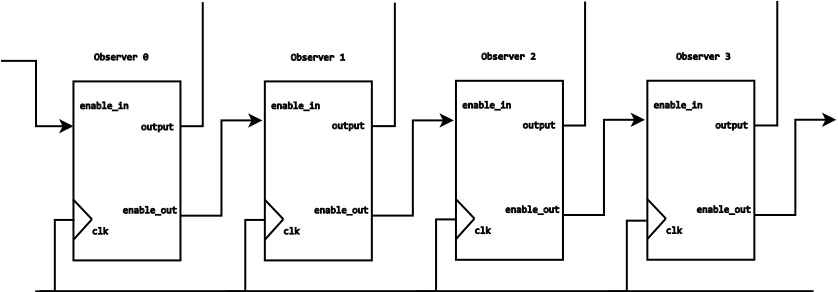
\includegraphics[width=450px]{Chapter2/Figs/Raster/Observer-stage.png}
\caption[Invariant Observer stages in cascade , m=4]{Example for m=4 Invariant Observer Stages concatenated in cascade. }
\label{fig:observerstages}
\end{figure}
\end{center}
This ensures that the observers are working delayed in the meaning of time.
The asynchronous part works immediately after every change of the system state.  
Signal \textbf{inc\_tau} increments the input signal \textbf{invariance\_tau},which represents $\tau+1$ at every execution time.
The process entity \textbf{comb\_cycle} is an internal clock counter which only counts up and down between values 0 and m.
The signal \textbf{cycle} is significant to check the condition ``(clock mod m) = 0'' from the Algorithm~\ref{alg:observerstage}.
The process entity \textbf{comb\_logic} implements the real part of the algorithm.
Signal \textbf{count\_p} will be incremented in each clock cycle until it reaches $\tau+1$.
The counter should be initialised with 0 (as indicated in the algorithm),but is incremented immediately every clock cycle,this also happens in the clock cycle where \textbf{count\_p}
should be reseted.
To show this fact we have the signal \textbf{count} initialised with 1. But this signal is only for reasoning and will be reduced by a syntheses tool.  
The synchronous design is in a way cumbersome,but this is because of the way how the states changes.
If the counter should be incremented after evaluation of some conditions,this doesn't mean an immediate change of the counter.
To overcome this handicap the counter is initialised with 2,this means we check at every clock cycle if counter count\_p will reach the maximum
at the next clock cycle. This enables us to change things on time. 
In \textbf{comb\_cycle},\textbf{count\_p} will be reseted only if signal $W(\phi)$ was evaluated as not active,according to the algorithm.
One Case is observed in the first if branch,if the clock passed m cycles or not. If a reset condition happens or \textbf{enable\_in}
is not active,than signal \textbf{enable\_logic} combines these two cases in one signal which leads the if query inside of \textbf{comb\_cycle} to the last branch,in case of \textbf{enable\_logic}
is not active. The other parts of \textbf{comb\_cycle} are straightforward,if you compare it with the algorithm.In case the counter \textbf{count\_p} reaches the maximum,
the  \textbf{output} of the observer stage is activated.\newline
Some points about the improvements made in that design,but it can also be seen as guidelines for further design cases.
It is very important that no Latches are built by the syntheses tool,so every if branch must contain the same changes on the same signals.
A further point is to reduce the number of if branches to a minimum. If branches inside of an If branch extends signal paths and reduce the maximum clock design of the whole design.
\newline
In the next chapter we get an overview of the Hardware Realisation of the current design,which shows us a more visual view on that.
